
\section{Automated Verification Framework}
\label{sec:methodology}
%-------------------------------------------------------------------------------


To systematically analyze the prevalence and impact of ghost citations, we first need a reliable method to identify them at scale.
To this end, we developed \citeb, an automated citation verification framework designed to robustly identify invalid citations across large corpora of academic papers.
In this section, we describe the design and implementation of our \citeb framework, detailing how it addresses the significant challenges of citation verification to enable our subsequent analyses.

%-------------------------------------------------------------------------------

\subsection{Framework Design}
\label{subsec:framework_design}

Verifying citations at scale raises several technical and practical challenges; we summarize these challenges below, then state the design goals we set to address them.

\noindent
\textbf{Design Challenges.}
\begin{itemize}
    % \xl{引用，比如google或者其他学术平台提供的引用格式}
    \item \textit{Parsing heterogeneity}: academic citations exhibit enormous format diversity, varying across venues, disciplines, and even individual papers; PDF extraction introduces additional noise through OCR errors, non-standard fonts, so a robust pipeline needs to tolerate parsing imperfections without generating excessive false positives.
    % \xl{这个结果要在后面的实验有一定的支撑，或者在这里脚注直接写一下统计，比如多少引用没有doi，最后有一个占比。
    \item \textit{Database coverage}: no single bibliographic database provides comprehensive coverage; different sources have different profiles, so absent results are often ambiguous, motivating a multi-source strategy.
    % xl{我们有做这个区分吗}
    \item \textit{Verification scalability}: verifying millions of citations requires a well-engineered framework design, such as rate limiting, cache reuse, and concurrent requests, to achieve practical throughput without excessive costs.
\end{itemize}

\noindent
\textbf{Design Goals.}
To address these challenges, we set the following design goals: (1)~This system should provide parsing robust to format heterogeneity that recovers from extraction failures. (2)~It should provide verification leveraging multiple sources in a cost-effective order and scaling to large corpora. (3)~It should remain robust to diverse citation formats to prevent legitimate references from being over-flagged as invalid
With these goals in mind, we developed \citeb, an automated citation verification framework.

\noindent
\textbf{Design Overview.}
With these challenges and goals, we designed \citeb as a modular, cascaded verification pipeline, as illustrated in \Cref{fig:methodology_overview}.
It follows a retrieval-first, error-tolerant pipeline to verify citations at scale. It parses noisy reference strings into structured metadata, queries a cascaded set of sources, and then classifies validity using similarity-based matching to tolerate minor metadata variations. 
The cascade prioritizes low-cost, high-precision sources and falls back to broader search only when needed, while an LLM reparser serves as a last-resort correction for malformed inputs. 
This design balances coverage and precision, ensuring that the system catches fabricated references without over-flagging legitimate citations.

%-------------------------------------------------------------------------------
\subsection{Framework Implementation}
\label{subsec:framework_impl}

\citeb is implemented as a three-stage pipeline: \textit{parsing}, \textit{verification}, and \textit{classification}; we describe each stage below.

\noindent
\textbf{Stage 1: Reference Parsing.}
The parsing stage aims to extract structured metadata from raw citation strings while robustly handling OCR errors and diverse citation formats.
% \xl{这里究竟是怎么fallback的，需要描述}
We employ a hybrid parser that combines standard PDF extraction with an LLM-based fallback: when the initial parsing leads to a verification failure, we re-parse and then re-run the verification chain with LLM-extracted metadata, ensuring high accuracy across varied parsing scenarios.

\noindent\textbf{Stage 2: Cascaded Verification.}
With structured metadata extracted, the verification stage checks citation validity using a cascaded strategy with four verification methods executed sequentially:

\begin{enumerate}
    \item \textit{CacheVerificationStrategy.}
    We first query a local SQLite database of previously verified citations.
    This cache stores results from prior searches, enabling efficient re-verification and reducing API costs.
    The cache is keyed by normalized title and returns stored verification results along with matched external reference metadata.
    
    \item \textit{AcademicDBVerificationStrategy.}
    For uncached entries, we query multiple bibliographic databases in cascade.
    We prioritize local academic databases for efficiency and reliability, then extend to broader search platforms when needed.
    The query is constructed from the citation title, and returned results are parsed to extract title, authors, year, and venue metadata. We store all results in the cache for future queries.
    % \xl{为什么只选title，这个需要在这里或者后面实现的地方有解释}

    \item \textit{WebSearchFallbackStrategy.}
    If the academic databases fail to find the reference, we fall back to general web search.
    This broader search covers recent papers not yet indexed by academic databases, technical reports, preprints, and non-traditional academic content.

    \item \textit{LLMReparseStrategy.}
    If all prior strategies fail to find a match, we hypothesize that parsing errors may have corrupted the search query.
    The system invokes the LLM reparser to re-extract metadata from the raw string, then re-executes the verification chain with the corrected metadata.
    This addresses cases where minor parsing errors, ensuring high accuracy even with noisy inputs.
\end{enumerate}

Each strategy returns either a \texttt{VerificationResult} (if verification succeeds or definitively fails), or triggers the next strategy in the cascade.

\noindent\textbf{Stage 3: Similarity-Based Classification.}
After retrieving candidate matches from the verification stage, we classify the citation as \texttt{Valid} or \texttt{Invalid} based on the similarity between the input citation and retrieved candidates.
In this part, we only focus on title similarity, as our preliminary goal is to identify citations that are untraceable or even non-existent (i.e. ghost citations), rather than citation errors as reported in prior work~\cite{simkin2005stochastic, simkin2003read},
The classfication is based on the highest similarity score among all retrieved candidates, using a empirical calibrated threshold $\theta$ to determine validity: if the maximum similarity exceeds $\theta$, we classify the citation as \texttt{Valid}; otherwise, it is classified as \texttt{Invalid}.

\subsection{Implementation Details}
We implement \citeb in Python with asynchronous I/O (asyncio) for concurrent API requests, enabling efficient parallel processing of multiple citations.
Below, we detail each key component.

\noindent\textbf{Parsing and Verification Services.}
For parsing, we use GROBID~\cite{grobid-client-python} as the primary parser and a Qwen3-Flash~\cite{bai2023qwen} based LLM reparser for cases with parsing failures, extracting structured metadata via a JSON schema.
For verification, we employ multiple sources: we construct a local DBLP database by parsing the DBLP XML dump, enabling efficient local verification queries; we also access Google Scholar and Google Search through the ScrapingDog API proxy~\cite{scrapingdog} for searching recent or non-indexed papers.

\noindent\textbf{Similarity Computation and Threshold Selection.}
For similarity-based classification, we normalize titles and compute Levenshtein distance\cite{levenshtein1966binary} (using the highest similarity among all retrieved candidates).
We set the classification threshold to $\theta = 0.9$, roughly corresponding to a one--two word difference in a long title.
We validate this choice based on the subsequent experiments in \cref{sec:llm_results} and \cref{sec:archival_results}, using the empirical CDF of title similarity for real-paper citations and LLM-generated citations (\Cref{fig:llm_papers_similarity_ecdf}).
Real-paper similarities remain near 1.0: only 0.4\% fall at or below 0.9, and the small tail below 1.0 is largely attributable to noise (OCR errors, hyphenation, minor typos).
In contrast, LLM-generated citations rise gradually, with 50.3\% at or below 0.9, validating $\theta = 0.9$ as a threshold that preserves high recall for real papers while filtering low-similarity hallucinations.
\begin{figure}[t]
    \centering
    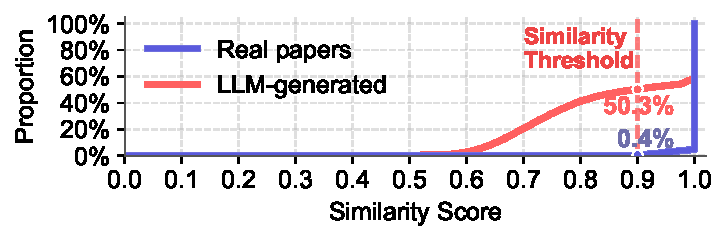
\includegraphics[width=\columnwidth]{Sec3_Methodology/llm_papers_similarity_ecdf.pdf}
    \vspace{-5.5mm}
\caption{ECDF of title similarity scores: LLM-generated vs.\ real-paper citations.}
    \label{fig:llm_papers_similarity_ecdf}
\end{figure}

%%%%%%%%%%%%%%%%%%%%%%%%%%%%%%%%%%%%%%%%%%%%%%%%%%%%%%%%%%%%%%%%%%%%%%%%%%%%%%%%
% JUSTIFICATION FOR DIFFERENTIAL THRESHOLDING IN CITATION VALIDATION
% ------------------------------------------------------------------------------
% This section provides the statistical rationale for applying a Similarity 
% Threshold of 1.0 for LLM-generated citations versus 0.9 for Real Papers.
%%%%%%%%%%%%%%%%%%%%%%%%%%%%%%%%%%%%%%%%%%%%%%%%%%%%%%%%%%%%%%%%%%%%%%%%%%%%%%%%

% 1. VALIDATION OF REAL PAPER THRESHOLD (Threshold = 0.9)
% ------------------------------------------------------------------------------
% Observation: The ECDF of 'Real papers' (green line) remains near zero until 
% reaching the [0.9, 1.0] interval, with a value of only 0.4% at x = 0.9.
%
% Rationale: 
% - The steep vertical jump at x > 0.9 indicates that 99.6% of real citations 
%   exhibit high fidelity to the ground truth.
% - The delta between 0.9 and 1.0 is categorized as 'Measurement Noise' 
%   (e.g., OCR character recognition errors, hyphenation, or minor typos).
% - Thus, 0.9 is a robust boundary that ensures high Recall by accommodating 
%   non-systematic technical artifacts without sacrificing validity.

% 2. VALIDATION OF LLM-GENERATED THRESHOLD (Threshold = 1.0)
% ------------------------------------------------------------------------------
% Observation: The ECDF of 'LLM-generated' (blue line) exhibits a gradual 
% slope starting from x = 0.6, with a cumulative value of ~54.1% at x < 1.0.
%
% Rationale: 
% - Unlike real papers, LLMs exhibit 'Structural Bias' rather than random noise.
% - The high density of citations in the [0.6, 0.99] range represents 
%   'Near-miss Hallucinations'—citations that appear semantically plausible 
%   but are factually non-existent or logically spliced.
% - Adopting a strict Exact Match (Similarity = 1.0) is mandatory to ensure 
%   High Precision, filtering out sophisticated hallucinations that would 
%   otherwise pass a 0.9 threshold.

% 3. STATISTICAL CONCLUSION
% ------------------------------------------------------------------------------
% The divergence between the quasi-binary distribution of Real Papers and the 
% continuous dispersion of LLM outputs justifies the use of an asymmetric 
% decision boundary. This prevents the inflation of LLM accuracy while 
% maintaining the empirical verifiability of human-authored research.
%%%%%%%%%%%%%%%%%%%%%%%%%%%%%%%%%%%%%%%%%%%%%%%%%%%%%%%%%%%%%%%%%%%%%%%%%%%%%%%%


\noindent\textbf{Practical Considerations.}
Key implementation choices include semaphore-based rate limiting (default: 10 concurrent requests) to respect API quotas; batch processing of entire directories with progress tracking and incremental result export; and CSV export with columns for final status, diagnosis, similarity scores, and matched external reference metadata.
Taken together, these design and engineering choices make \citeb a practical, scalable, and robust verification system for large-scale citation analysis, enabling both our subsequent experiments and real-world deployment.

% The framework processes approximately 500 citations per hour with the default concurrency settings, limited primarily by API rate limits rather than computational overhead.

%-------------------------------------------------------------------------------

